% Belvu User Manual
% Author: Gemma Barson
%
% Run the following command twice to create a pdf of this manual
% (two runs are necessary to make sure all of the cross-references
% are up to date):
%
%    pdflatex Belvu_manual.tex
%
% This file was converted to LaTeX by Writer2LaTeX ver. 1.0.2
% see http://writer2latex.sourceforge.net for more info
%
\documentclass[letterpaper]{article}
\usepackage[latin1]{inputenc}
\usepackage[T1]{fontenc}
\usepackage[english]{babel}
\usepackage{amsmath}
\usepackage{amssymb,amsfonts,textcomp}
\usepackage{color}
\usepackage{array}
\usepackage{supertabular}
\usepackage{hhline}
\usepackage{hyperref}
\usepackage{titlesec}
\hypersetup{pdftex, colorlinks=true, linkcolor=blue, citecolor=blue, filecolor=blue, urlcolor=blue, pdftitle=Belvu User Manual, pdfauthor=Gemma Barson, pdfsubject=, pdfkeywords=}
\usepackage[pdftex]{graphicx}
% Paragraph styles
\setlength{\parindent}{0pt}
% Text styles
\newcommand\textstyleInternetlink[1]{\textcolor{blue}{#1}}
\newcommand\textstyleSourceText[1]{\texttt{#1}}
\newcommand\textstyleFootnoteSymbol[1]{\textsuperscript{#1}}
\definecolor{darkblue}{rgb}{0.2,0.3,0.5}
\definecolor{lightblue}{rgb}{0.3,0.5,0.8}
%\DeclareFixedFont{\sectionfont}{T1}{phv}{bx}{n}{16pt}
%\DeclareFixedFont{\subsectionfont}{T1}{phv}{bx}{n}{14pt}
%\DeclareFixedFont{\subsubsectionfont}{T1}{phv}{bx}{n}{12pt}
\titleformat{\section} {\normalfont\LARGE\bf\color{darkblue}}{\thesection}{1em}{}
\titleformat{\subsection} {\normalfont\large\bf\color{lightblue}}{\thesubsection}{1em}{}
\titleformat{\subsubsection} {\normalfont\normalsize\bf\color{lightblue}}{\thesubsubsection}{1em}{}
% Outline numbering
\setcounter{secnumdepth}{0}
\makeatletter
\newcommand\arraybslash{\let\\\@arraycr}
\makeatother
% List styles
\newcommand\liststyleLi{%
\renewcommand\labelitemi{{\textbullet}}
\renewcommand\labelitemii{{\textbullet}}
\renewcommand\labelitemiii{{\textbullet}}
\renewcommand\labelitemiv{{\textbullet}}
}
\newcommand\liststyleLii{%
\renewcommand\labelitemi{{\textbullet}}
\renewcommand\labelitemii{{\textbullet}}
\renewcommand\labelitemiii{{\textbullet}}
\renewcommand\labelitemiv{{\textbullet}}
}
\newcommand\liststyleLiii{%
\renewcommand\labelitemi{{\textbullet}}
\renewcommand\labelitemii{{\textbullet}}
\renewcommand\labelitemiii{{\textbullet}}
\renewcommand\labelitemiv{{\textbullet}}
}
\newcommand\liststyleWWviiiNumxxxvi{%
\renewcommand\labelitemi{{\textbullet}}
\renewcommand\labelitemii{o}
\renewcommand\labelitemiii{[F0A7?]}
\renewcommand\labelitemiv{[F0B7?]}
}
\newcommand\liststyleLiv{%
\renewcommand\labelitemi{{\textbullet}}
\renewcommand\labelitemii{${\circ}$}
\renewcommand\labelitemiii{${\blacksquare}$}
\renewcommand\labelitemiv{{\textbullet}}
}
\newcommand\liststyleWWviiiNumxxxi{%
\renewcommand\theenumi{\arabic{enumi}}
\renewcommand\theenumii{\alph{enumii}}
\renewcommand\theenumiii{\roman{enumiii}}
\renewcommand\theenumiv{\arabic{enumiv}}
\renewcommand\labelenumi{\theenumi.}
\renewcommand\labelenumii{\theenumii.}
\renewcommand\labelenumiii{\theenumiii.}
\renewcommand\labelenumiv{\theenumiv.}
}
\newcommand\liststyleWWviiiNumxxxv{%
\renewcommand\labelitemi{{\textbullet}}
\renewcommand\labelitemii{o}
\renewcommand\labelitemiii{[F0A7?]}
\renewcommand\labelitemiv{[F0B7?]}
}
\newcommand\liststyleWWviiiNumxiii{%
\renewcommand\labelitemi{{\textbullet}}
\renewcommand\labelitemii{o}
\renewcommand\labelitemiii{[F0A7?]}
\renewcommand\labelitemiv{[F0B7?]}
}
\newcommand\liststyleWWviiiNumxxvii{%
\renewcommand\labelitemi{{\textbullet}}
\renewcommand\labelitemii{o}
\renewcommand\labelitemiii{[F0A7?]}
\renewcommand\labelitemiv{[F0B7?]}
}
\newcommand\liststyleWWviiiNumxxvi{%
\renewcommand\labelitemi{{\textbullet}}
\renewcommand\labelitemii{o}
\renewcommand\labelitemiii{[F0A7?]}
\renewcommand\labelitemiv{[F0B7?]}
}
\newcommand\liststyleWWviiiNumxvi{%
\renewcommand\labelitemi{{\textbullet}}
\renewcommand\labelitemii{o}
\renewcommand\labelitemiii{[F0A7?]}
\renewcommand\labelitemiv{[F0B7?]}
}
\newcommand\liststyleWWviiiNumxxxvii{%
\renewcommand\labelitemi{{\textbullet}}
\renewcommand\labelitemii{o}
\renewcommand\labelitemiii{[F0A7?]}
\renewcommand\labelitemiv{[F0B7?]}
}
\newcommand\liststyleWWviiiNumxx{%
\renewcommand\labelitemi{{\textbullet}}
\renewcommand\labelitemii{o}
\renewcommand\labelitemiii{[F0A7?]}
\renewcommand\labelitemiv{[F0B7?]}
}
% Page layout (geometry)
\setlength\voffset{-1in}
\setlength\hoffset{-1in}
\setlength\topmargin{2.54cm}
\setlength\oddsidemargin{3.175cm}
\setlength\textheight{21.363003cm}
\setlength\textwidth{15.240001cm}
\setlength\footskip{1.497cm}
\setlength\headheight{0cm}
\setlength\headsep{0cm}
% Footnote rule
\setlength{\skip\footins}{0.119cm}
\renewcommand\footnoterule{\vspace*{-0.018cm}\setlength\leftskip{0pt}\setlength\rightskip{0pt plus 1fil}\noindent\textcolor{black}{\rule{0.25\columnwidth}{0.018cm}}\vspace*{0.101cm}}
% Pages styles
\makeatletter
\newcommand\ps@Standard{
  \renewcommand\@oddhead{}
  \renewcommand\@evenhead{}
  \renewcommand\@oddfoot{\thepage{}}
  \renewcommand\@evenfoot{\@oddfoot}
  \renewcommand\thepage{\arabic{page}}
}
\newcommand\ps@FirstPage{
  \renewcommand\@oddhead{}
  \renewcommand\@evenhead{}
  \renewcommand\@oddfoot{}
  \renewcommand\@evenfoot{}
  \renewcommand\thepage{\arabic{page}}
}
\makeatother
\pagestyle{Standard}
\setlength\tabcolsep{1mm}
\renewcommand\arraystretch{1.3}
% footnotes configuration
\makeatletter
\renewcommand\thefootnote{\arabic{footnote}}
\makeatother
\newcounter{Figure}
\renewcommand\theFigure{\arabic{Figure}}

\title{Belvu User Manual}
\author{Gemma Barson\\Wellcome Trust Sanger Institute\\gemma.barson@sanger.ac.uk}
\date{2011-09-22}

\begin{document}

\thispagestyle{FirstPage}
{\centering\sffamily\bfseries\color[rgb]{0.0,0.27058825,0.5254902}
\Huge\bf{Belvu User Manual}
\par}

\bigskip

{\centering
\large{Written by Gemma Barson}
\par}
{\centering
{\textless}\href{mailto:gb10@sanger.ac.uk}{gb10@sanger.ac.uk}{\textgreater}
\par}

\bigskip

{\centering
\large{Wellcome Trust Sanger Institute}
\par}
{\centering
22 September 2011
\par}


\clearpage\section[Revision History]{Revision History}

\begin{center}
\tablehead{}
\begin{supertabular}{|m{8.073cm}|m{3.2849998cm}|m{3.282cm}|}
\hline
\bf Revision &
\bf Date &
\bf Author\\\hline
First revision (Belvu v4.4.1) &
18/01/11 &
Gemma Barson\\\hline
Updated for version 4.14 &
02/07/12 &
Gemma Barson\\\hline
\end{supertabular}
\end{center}

\clearpage
\tableofcontents

\clearpage\section[Introduction]{Introduction}
This manual explains how to configure, run and use Belvu. \ Belvu is a multiple sequence alignment viewer and phylogenetic tool. It has an extensive set of user-configurable modes to color residues by conservation or by residue type, and some basic alignment editing capabilities. It can generate distance matrices between sequences and construct distance-based trees, either graphically or as part of a phylogenetic software pipeline.

Key features include:

\begin{itemize}
\item Residues can be coloured by conservation, with user-configurable cutoffs and colours.
\item Residues can be coloured by residue type (user-configurable).
\item Colour schemes can be imported or exported.
\item Swissprot (or PIR) entries can be fetched by double clicking.
\item The position in the alignment can be easily tracked.
\item Simple editing commands for rows and columns is supported (although Belvu is not intended to be a full editor).
\item The alignment can be saved in Stockholm, Selex, MSF or FASTA format.
\item Distance matrices between sequences can be generated using a variety of distance metrics.
\item Distance matrices can be imported or exported.
\item Trees can be constructed based on various distance-based tree reconstruction algorithms.
\item Trees can be saved in New Hampshire format.
\item Belvu can perform bootstrap phylogenetic reconstruction.
\item Belvu can be used as a graphical tree viewer, or as a command-line tool for use in phylogenetic software pipelines.
\end{itemize}

Belvu is maintained by the Wellcome Trust Sanger Institute and is available as part of the SeqTools package. \ The software can be downloaded from the Sanger Institute{\textquoteright}s website: 

\href{http://www.sanger.ac.uk/resources/software/seqtools/}
{\textstyleInternetlink{http://www.sanger.ac.uk/resources/software/seqtools}}

\clearpage\section[Getting Started]{Getting Started}
\subsection[Running Belvu]{Running Belvu}
As a minimum, Belvu takes the following required arguments:
\begin{quote}
\begin{verbatim}belvu <alignment_file>
\end{verbatim}
\end{quote}
 where {\textless}alignment\_file{\textgreater} is a file or pipe containing the multiple alignment in Stockholm, Selex, MSF or aligned-Fasta format (see below).

Run {\textquoteleft}belvu{\textquoteleft} without any arguments to see brief usage information, or, for more detailed help, run:
\begin{quote}
\begin{verbatim}
belvu --help 
\end{verbatim}
\end{quote}

\subsection[File formats]{File formats}
Belvu currently supports Stockholm (Mul/Pfam), Selex, MSF and aligned- and unaligned Fasta formats. \ Belvu will automatically detect which file format is supplied. \ The {\textquotesingle}raw{\textquotesingle} file format can also be used, but you must pass a raw file using the {\textasciigrave}-r{\textasciigrave} argument because Belvu cannot detect this format automatically.

\subsubsection[Selex]{Selex}
Selex is the native format used by Sean Eddy{\textquotesingle}s HMM package HMMER. \ For details, see:

http://www.psc.edu/general/software/packages/hmmer/manual/node46.html.

\bigskip

Each line contains a name, followed by the aligned sequence. A space, dash, underscore, or period denotes a gap. If the alignment is too long to fit on one line, the alignment is split into multiple blocks, separated by blank lines. The number of sequences, their order, and their names must be the same in every block (even if a sequence has no residues in a given block!) Other blank lines are ignored. You can add comments to the file on lines starting with a \#.

\begin{quote}
\begin{verbatim}
seq1 \ \ \ \ ACGACGACGACG.
seq2 \ \ \ \ ..GGGAAAGG.GA
seq3 \ \ \ \ UUU..AAAUUU.A
seq1 \ ..ACG
seq2 \ AAGGG
seq3 \ AA...UUU
\end{verbatim}
\end{quote}

\subsubsection[Stockholm]{Stockholm}
Also known as {\textquotedblleft}Mul{\textquotedblright} or {\textquotedblleft}Pfam{\textquotedblright} format, Stockholm is the native format used by Pfam and Rfam to disseminate protein and RNA sequence alignments. \ The file must start with a line giving the format version, and end with {\textasciigrave}//{\textasciigrave}. \ It has one domain per line:

\begin{quote}
\begin{verbatim}
# STOCKHOLM 1.0
<sequence_name>/<start>-<end> <sequence>
...
//
\end{verbatim}
\end{quote}

The residues must be aligned and gaps should be represented by dots. \ Markup lines can also be included; see http://en.wikipedia.org/wiki/Stockholm\_format for more details.

\subsubsection[MSF]{MSF}
Note on the MSF format: The {\textquotedbl}..... Check: ..{\textquotedbl} line has to come before the first line that does not start with a space. The only legal exception is the line {\textquotedbl}PileUp of:{\textquotedbl} from GCG programs.

\begin{quote}
\begin{verbatim}
[Pileup]

[<filename>]   MSF:  <len>  Type: <type>    Check:  <check>   ..

 Name: <name1>  Len:  <len>  Check:  <check>  Weight:  <weight>
 Name: <name2>  Len:  <len>  Check:  <check>  Weight:  <weight>
 ...
//
<name1>      <sequence>
<name2>      <sequence>
...
<name1>      <sequence>
<name2>      <sequence>
...
\end{verbatim}
\end{quote}

The sequence names can include coordinates, e.g.

\begin{quote}
\begin{verbatim}
<name>/<start>-<end>
\end{verbatim}
\end{quote}

\subsubsection[Fasta]{Fasta}
In Fasta format, the sequence name is on a line starting with {\textasciigrave}{\textgreater}{\textasciigrave}, and the sequence on the following line(s). \ Input files for Belvu must be in aligned-Fasta format, where gaps are included so that each sequence is the same length.

\begin{quote}
\begin{verbatim}
>seq1
ACGACGACGACG.
..ACG
>seq2
..GGGAAAGG.GA
AAGGG
\end{verbatim}
\end{quote}

Belvu does not accept unaligned-Fasta files as input, but can output the sequences in unaligned Fasta format (i.e. with gaps removed)

\subsubsection[Raw]{Raw}
The raw file format is as follows. \ Raw files must be passed using the {\textasciigrave}-r{\textasciigrave} command line argument because Belvu cannot detect this file format automatically.

\begin{quote}
\begin{verbatim}
<name> <sequence>
<name> <sequence>
...
\end{verbatim}
\end{quote}

\section[The Belvu Windows]{The Belvu Windows}
\subsection[Main window]{Main window}
The main Belvu window contains the alignments. \ Residues are coloured by conservation or by residue type; use the Color menu to change the colour scheme.

\begin{figure}[htb]
\centering
\color{lightblue}
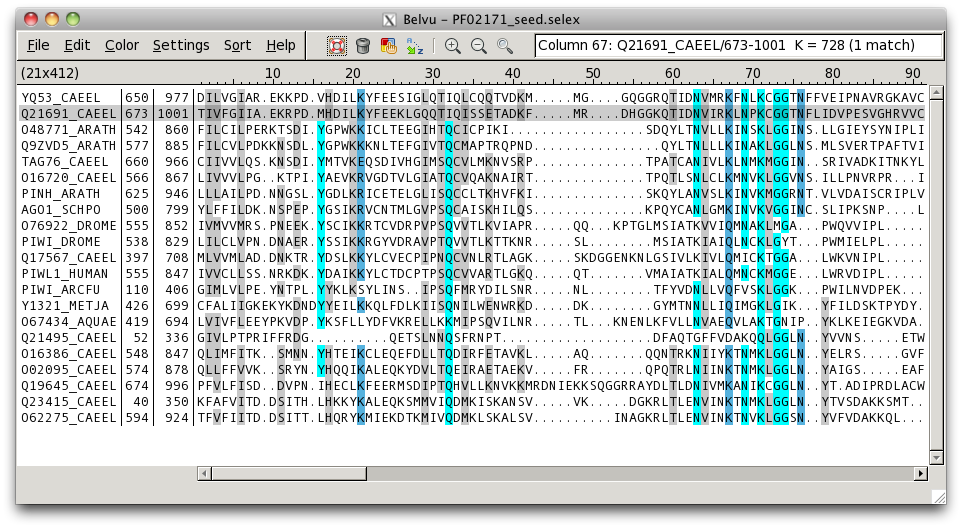
\includegraphics[width=\textwidth]{img_window_alignment_by_conservation.png}
\caption{Alignment window in colour-by-conservation mode}
\label{fig:belvu_cons}
\end{figure}


\begin{figure}[htb]
\centering
\color{lightblue}
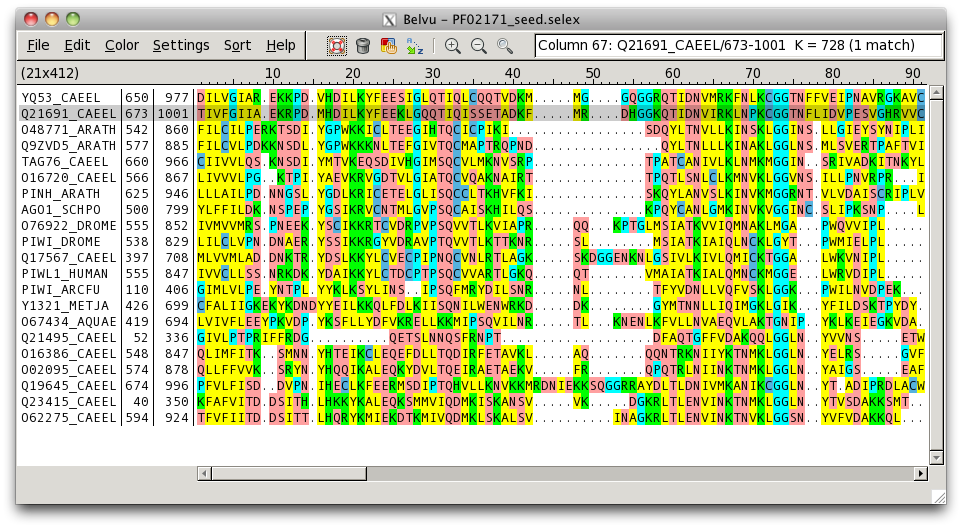
\includegraphics[width=\textwidth]{img_window_alignment_by_residue.png}
\caption{Alignment window in colour-by-residue mode}
\label{fig:belvu_residue}
\end{figure}

At the top of the alignment list is a header displaying the number of sequences and alignment length, e.g.
\begin{quote}
\begin{verbatim}
(21x412)
\end{verbatim}
\end{quote}
means there are 21 sequences and the alignment length is 412.

\bigskip

The alignment list contains the following columns:

\begin{supertabular}{>{\bfseries}l l}
Name &
The sequence name\\
Start &
The start coordinate in the match sequence\\
End &
The end coordinate in the match sequence\\
Score &
Only displayed if a scores file was loaded; displays the score of the sequence\\
Sequence &
Displays the sequence data\\
\end{supertabular}

\subsubsection[Selections]{Selections}
Click on a row to select that alignment. \ Details about the selected row will be shown in the feedback box on the toolbar. \ If there are other sequences with the same name, their names will be highlighted in the alignment list (but only the clicked row will have the whole row highlighted). \ The number of matches is shown in brackets in the feedback box.

If you clicked within the sequence area, a column will also be selected; the column number (1-based from the left) that you clicked will be shown in the feedback box, along with the residue and the sequence coordinate at that column for the selected sequence.

Middle-click in the alignment in order to select a column; the current column will be highlighted while the middle button remains pressed and you can drag to other columns to see column information dynamically. \ When you release the mouse button, the display will scroll so that it is centered on the selected column.

\subsubsection[Fetching sequences]{Fetching sequences}
Double-click on a row in the alignment to fetch that sequence; the program used to fetch sequences must be specified in the BELVU\_FETCH environment variable before Belvu is opened, e.g. in a C shell terminal:

\begin{quote}
\begin{verbatim}
setenv BELVU\_FETCH {\textquotesingle}pfetch -F{\textquotesingle}
\end{verbatim}
\end{quote}

\subsubsection[Toolbar]{Toolbar}
The toolbar contains shortcuts to several of the menu items, as well as a feedback area displaying information about the currently-selected row and/or column.


\begin{figure}[htb]
\centering
\color{lightblue}

\includegraphics[width=\textwidth]{img_toolbar.png}
\caption{The toolbar}
\label{fig:toolbar}
\end{figure}

The toolbar buttons are as follows:

\begin{supertabular}{>{\bfseries}p{0.4\textwidth} p{0.6\textwidth}}
Help &
Display the help pages. See the Help menu\\
Remove many sequences &
Start the mode that allows you to double-click to remove sequences. \ Click again or press Esc to cancel this mode. \ See the Edit menu\\
Edit current colour scheme &
Edit the current colour scheme (see the Color menu)\\
Sort alphabetically &
Sort sequences by name (see the Sort menu)\\
Zoom in &
Increase the font size in the alignment list\\
Zoom out &
Decrease the font size in the alignment list\\
Find &
Open the Find dialog\\
\end{supertabular}

\bigskip

The feedback area on the toolbar displays the following information:

\begin{supertabular}{>{\bfseries}p{0.4\textwidth} p{0.6\textwidth}}
Column {\textless}column{\textgreater}: &
If a column is selected, this displays the column number (1-based from the left-most column)\\
{\textless}name{\textgreater}/{\textless}start{\textgreater}-{\textless}end{\textgreater} &
If a sequence is selected, this displays the sequence name and its start/end coordinates\\
{\textless}residue{\textgreater} = {\textless}coord{\textgreater} &
If a column and sequence are selected, this displays the residue and coordinate of that column within that sequence\\
({\textless}n{\textgreater} match[s]) &
If a sequence is selected, this shows the number of sequences in the alignment with the same name (1 ={\textgreater} only the current sequence has that name)\\
\end{supertabular}


\subsubsection[Find dialog]{Find dialog}
The Find dialog allows you to search for sequences by name. \ Open it by clicking on the toolbar icon or by using the keyboard shortcut Ctrl-F.


\begin{figure}[htb]
\centering
\color{lightblue}
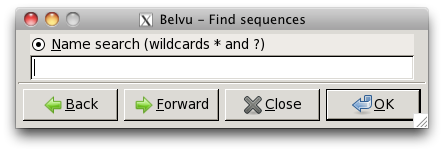
\includegraphics[width=10cm]{img_dialog_find_sequences.png}
\caption{Find-sequences dialog}
\label{fig:find_seqs}
\end{figure}

Enter the text you wish to search for. \ The text can include the wildcards {\textquotesingle}*{\textquotesingle} (for any amount of any character) or {\textquotesingle}?{\textquotesingle} (for one occurrence of any character).

Hit OK to close the dialog and search. \ If found, the first matching result will be highlighted in the alignment list. \ Alternatively, click Forward or Back on the Find dialog to perform a search forwards or backwards from the last search result. \ (These operations will start from the beginning of the list if there was no previous search result.)

\subsection[Tree]{Tree}
The tree window can be opened from the main window using the {\textquotesingle}Show tree{\textquotesingle} option on the File menu. \ The tree window will show a distance-based phylogenetic tree of the current alignment using the default settings. \ To edit the tree settings before calculating the tree, first select the {\textquotesingle}Tree settings{\textquotesingle} option from the File menu.

Click on a sequence name to select a sequence in the tree; the sequence will be highlighted in both the tree and the main window.

Click on a branch to either swap the nodes or re-root the tree from that branch; see the Tree settings section for more details.

\begin{figure}[htb]
\centering
\color{lightblue}
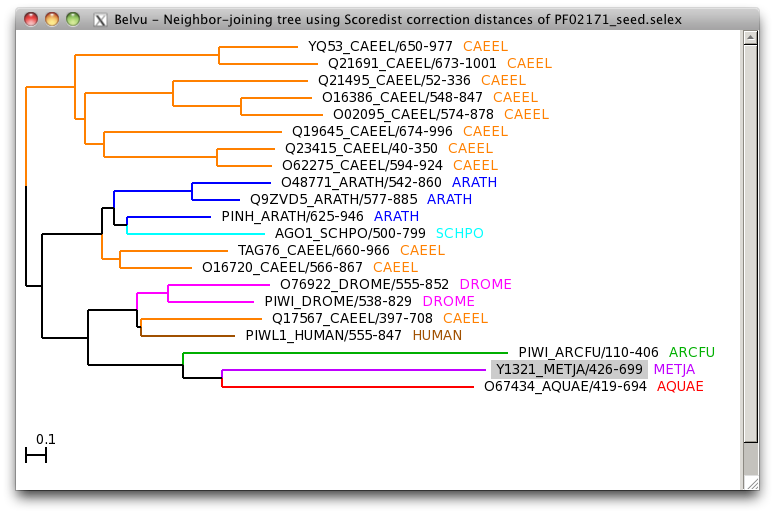
\includegraphics[width=\textwidth]{img_window_tree.png}
\caption{Tree window}
\label{fig:tree_window}
\end{figure}


\subsubsection[Tree menu]{Tree menu}
The tree menu can be accessed by right-clicking anywhere in the tree window.

\begin{figure}[htb]
\centering
\color{lightblue}
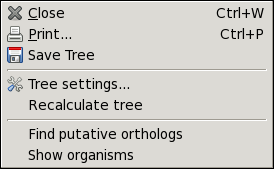
\includegraphics[width=6cm]{img_menu_tree.png}
\caption{Tree menu}
\label{fig:tree_menu}
\end{figure}

The options on the tree menu are as follows:

\begin{supertabular}{>{\bfseries}p{0.2\textwidth} p{0.8\textwidth}}
Close &
Close the tree window (the tree will not be deleted and can be opened again without recalculating)\\
Print &
Print the tree window\\
Save Tree &
Save the tree in New Hampshire format\\
Tree settings &
Open the tree settings dialog\\
Recalculate tree &
Forces the tree to be recalculated; this is required after the alignment has changed and the tree is now invalid (e.g. if rows have been deleted)\\
Find putative orthologs &
Highlights putative orthologs in the tree and outputs their details to the terminal\\
Show organisms &
Opens a window showing the list of organisms, and outputs the number of organisms to the terminal\\
\end{supertabular}


\subsubsection[Organisms window]{Organisms window}
Select {\textquotesingle}Show organisms{\textquotesingle} from the right-click menu in the tree to display the organisms window, which lists all of the organisms in the alignment: 

\begin{figure}[htb]
\centering
\color{lightblue}
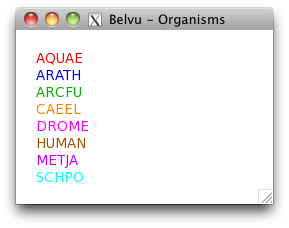
\includegraphics[width=6cm]{img_window_organisms.png}
\caption{Organisms window}
\label{fig:organisms}
\end{figure}


\subsubsection[Tree settings]{Tree settings}
\label{bkm:RefHeading45661104073125}To open the tree-settings dialog, use the {\textquotesingle}Tree settings{\textquotesingle} option from the File menu on the main window or from the right-click menu on the tree window.

\begin{figure}[htb]
\centering
\color{lightblue}
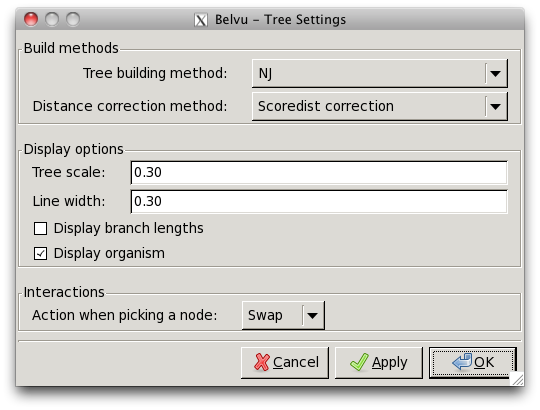
\includegraphics[width=13cm]{img_dialog_settings.png}
\caption{Tree settings dialog}
\label{fig:tree_settings}
\end{figure}

The options are as follows. \ Note that changing the tree building method or distance correction method will force the tree to be recalculated, which may take a long time for large alignments.

\begin{supertabular}{>{\bfseries}p{0.4\textwidth} p{0.6\textwidth}}
Tree building method &
Choose whether the tree should be built using the neighbour-joining or UPGMA method\\
Distance correction method &
Select the distance-correction method to use\\
Tree scale &
Adjust the horizontal scale used to draw the tree; set a smaller number to decrease the width of the tree or a larger number to increase it.\\
Line width &
Set the line width to use for the branches (0.1 ={\textgreater} 1 pixel)\\
Display branch lengths &
Whether to label branches with their lengths\\
Display organism &
Whether to display the organism next to the sequence name\\
Action when picking a node &
Swap: when you click a branch, its two child nodes will be swapped

Reroot: when you click a branch, the tree will be re-rooted with that node as the root

Note: to revert to the original tree, select the {\textquotesingle}Recalculate tree{\textquotesingle} option from the right-click menu\\
\end{supertabular}


\subsection[Conservation plot ]{Conservation plot }
To display the conservation profile, select {\textquotesingle}Show conservation plot{\textquotesingle} from the File menu. \ The conservation profile window will open displaying a plot of the conservation (vertical axis) against the column numbers (horizontal axis). \ The average conservation is shown as a red line.

\begin{figure}[htb]
\centering
\color{lightblue}
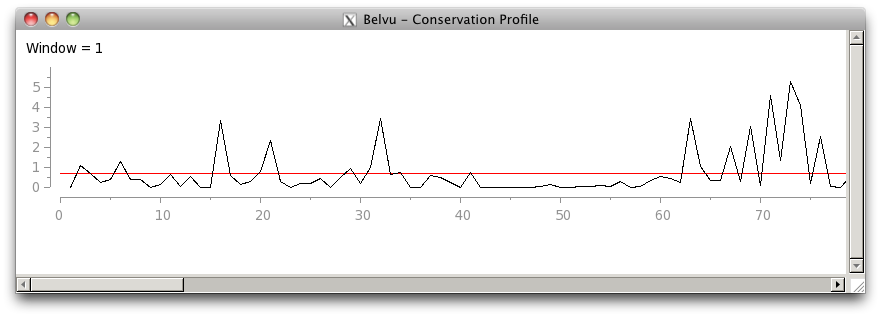
\includegraphics[width=\textwidth]{img_window_conservation_plot.png}
\caption{Conservation plot}
\label{fig:cons_plot}
\end{figure}


\subsubsection[Conservation plot menu]{Conservation plot menu}
Right-click anywhere on the conservation plot to display the menu:


\begin{figure}[htb]
\centering
\color{lightblue}
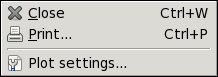
\includegraphics[width=6cm]{img_menu_conservation_plot.png}
\caption{Conservation plot menu}
\label{fig:cons_plot_menu}
\end{figure}

The options are:

\begin{supertabular}{>{\bfseries}l l}
Close &
Close the conservation plot window\\
Print &
Print the conservation plot\\
Plot settings &
Show the plot settings dialog\\
\end{supertabular}


\subsubsection[Conservation plot settings]{Conservation plot settings}
Select the {\textquotesingle}Plot settings{\textquotesingle} option from the right-click menu on the conservation plot to show the plot settings dialog:


\begin{figure}[htb]
\centering
\color{lightblue}
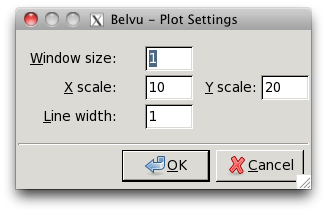
\includegraphics[width=0.5\textwidth]{img_dialog_plot_settings.png}
\caption{Conservation plot settings}
\label{fig:cons_plot_settings}
\end{figure}


The options are:

\begin{supertabular}{>{\bfseries}p{0.2\textwidth} p{0.8\textwidth}}
Window size &
Specify the size of the sliding window used to smooth out the curve; set a larger value for a smoother curve. \ The minimum value is 1, which means no smoothing is done\\
X scale &
Adjust the scale of the horizontal axis; set a smaller value to compress the scale or a larger value to expand it\\
Y scale &
Adjust the scale of the vertical axis; set a smaller value to compress the scale or a larger value to expand it\\
Line width &
Set the line width to use for the drawing, in pixels\\
\end{supertabular}


\section[Main menu]{Main menu}
The main menu can be accessed via the menu-bar at the top of the main window. \ Right-clicking in the main window is a shortcut to the File menu.

Note that menus with a dotted line at the top can be {\textquotedblleft}torn off{\textquotedblright} by clicking on the dotted line. \ A torn-off menu will stay visible on top of the Belvu window and can be repositioned by dragging its header bar. \ Click the dotted line again to get rid of it. 

\begin{figure}[htb]
\centering
\color{lightblue}
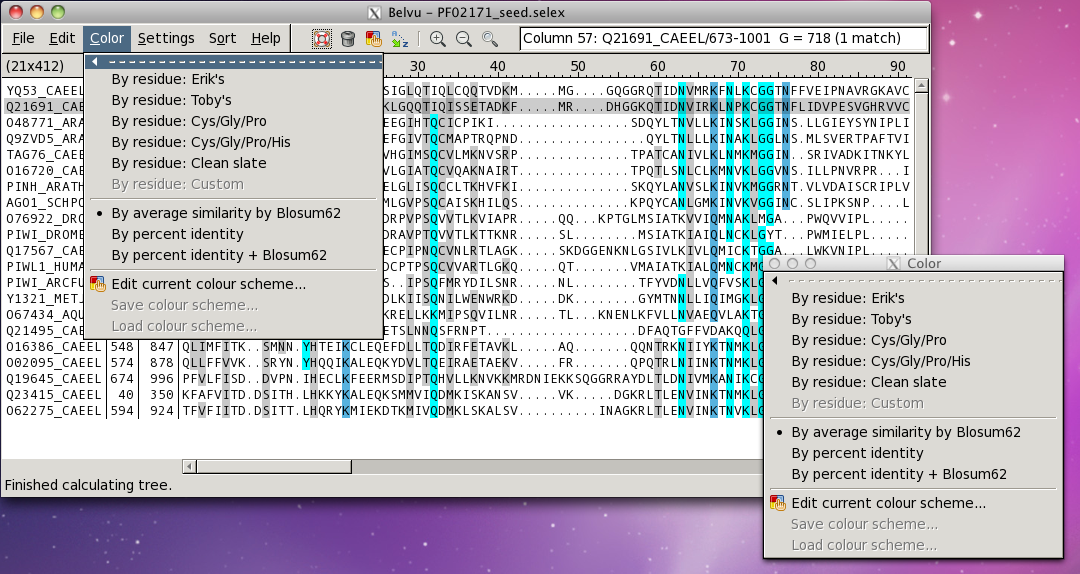
\includegraphics[width=\textwidth]{img_menu_tear_offs.png}
\caption{Menu tear-offs}
\label{fig:menu_tear_offs}
\end{figure}


\subsection[File menu]{File menu}

\begin{figure}[htb]
\centering
\color{lightblue}
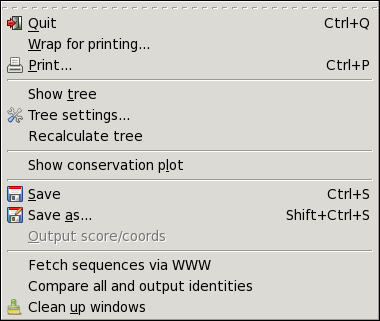
\includegraphics[width=10.3cm]{img_menu_file.png}
\caption{File menu}
\label{fig:file_menu}
\end{figure}


\begin{supertabular}{>{\bfseries}p{0.3\textwidth} p{0.7\textwidth}}
Quit  &
Quit Belvu (close all windows and exit)\\
Wrap for printing &
Open a window showing a wrapped alignment, suitable for printing\\
Print &
Print the current window (note that you should use the print option from the wrapped-alignment window to print the wrapped view)\\
Show tree &
Open the tree window; calculates the tree if it has not yet been calculated\\
Tree settings  &
Edit the settings used to calculate and display the tree\\
Recalculate tree  &
Use this to recalculate the tree after making changes that invalidate it, e.g. deleting rows\\
Show conservation plot  &
Show the conservation plot window\\
Save  &
Save the alignment in the current format\\
Save as  &
Save the alignment; allows you to select a different file format and choose \ whether coordinates should be saved and what separator character to use\\
Output score/coords  &
Only applicable if scores are loaded; outputs the score and coordinates of the currently-selected sequence to the terminal\\
Fetch sequences via WWW  &
Enables fetching of sequences over HTTP\\
Compare all and output identities  &
Compares each sequence against each other and outputs their identity and score to the terminal, along with some summary information about the maximum, minimum and mean score and identity\\
Clean up windows  &
Close all windows opened by this instance of Belvu (does not close the main window)\\
\end{supertabular}


\subsection[Edit menu]{Edit menu}



\begin{figure}[htb]
\centering
\color{lightblue}
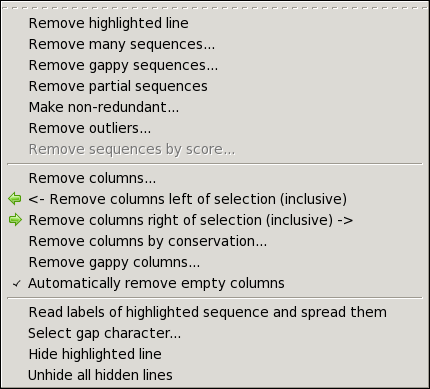
\includegraphics[width=11.6cm]{img_menu_edit.png}
\caption{Edit menu}
\label{fig:edit_menu}
\end{figure}


\begin{supertabular}{>{\bfseries}p{0.4\textwidth} p{0.6\textwidth}}
Remove highlighted line  &
Remove the currently-selected line\\
Remove many sequences  &
Enables a mode where you can double-click on sequences to remove them. The cursor will change to indicate that you are in this mode. Select the option again, press the Esc key, or right-click to cancel this mode\\
Remove gappy sequences  &
Remove sequences that have more than a given percentage of gaps\\
Remove partial sequences  &
Removes partial sequences\\
Make non-redundant  &
Remove sequences that are more than a given percentage identical to any other\\
Remove outliers  &
Remove sequences that are less than a given percentage identical to any other\\
Remove sequences by score  &
Only applicable if scores are loaded; remove sequences that have a score lower than a given threshold\\
Remove columns  &
Remove a specific range of columns\\
Remove columns left of selection  &
Removes the columns to the left of the currently-selected column (which is displayed in the feedback box on the toolbar, if a column is selected). \ The operation is inclusive, so the currently-selected column will be removed as well\\
Remove columns right of selection  &
Removes the columns to the right of the currently-selected column. The operation is inclusive, so the currently-selected column will be removed as well\\
Remove columns by conservation  &
Remove columns with a maximum conservation between specified values\\
Remove gappy columns  &
Remove columns with more than a given percentage of gaps\\
Automatically remove empty columns  &
After deleting sequences, columns that are left empty are automatically removed if this option is enabled\\
Read labels of highlighted sequence and spread them  &
Undocumented\\
Select gap character  &
Change the character used to display gaps in the alignment\\
Hide highlighted line  &
Hides the currently-selected line\\
Unhide all lines  &
Show all lines that were previously hidden\\
\end{supertabular}


\subsection[Color menu]{Color menu}


\begin{figure}[htb]
\centering
\color{lightblue}
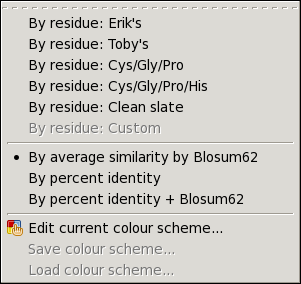
\includegraphics[width=0.5\textwidth]{img_menu_colour.png}
\caption{Colour menu}
\label{fig:color_menu}
\end{figure}

\begin{supertabular}{>{\bfseries}p{0.4\textwidth} p{0.6\textwidth}}
Erik{\textquotesingle}s &
Use Erik{\textquotesingle}s original built-in residue colour scheme\\
Toby{\textquotesingle}s &
Another built-in residue colour scheme\\
Cys/Gly/Pro &
A colour-by-residue scheme where only cystine, glycine and proline are highlighted\\
Cys/Gly/Pro/His &
A colour-by-residue scheme where only cystine, glycine, proline and histidine are highlighted\\
Clean slate &
Clear all colours; used for when you want to create a new colour scheme starting with all colours being white\\
Custom &
This option will become enabled when a residue colour scheme has been customised by editing it or loading it from file; if you change to a different colour scheme, you can toggle back to the custom colour scheme by selecting this option\\
By average similarity by Blosum62 &
A colour-by-conservation scheme colouring by average similarity by Blosum62\\
By percent identity &
A colour-by-conservation scheme colouring by percent identity\\
By percent identity + Blosum62 &
A colour-by-conservation scheme colouring by both percent identity and average similarity by Blosum62\\
Edit current colour scheme &
Edit the current colour scheme. \ If in colour-by-residue mode, allows you to edit the residue colours; if in colour-by-conservation mode, allows you to edit the thresholds and colours for the different levels of conservation\\
Save colour scheme &
Only applicable in colour-by-residue mode; save the current colour scheme to file\\
Load colour scheme &
Only applicable in colour-by-residue mode; load a colour scheme from file\\
\end{supertabular}


\subsection[Settings menu]{Settings menu}

\begin{figure}[htb]
\centering
\color{lightblue}
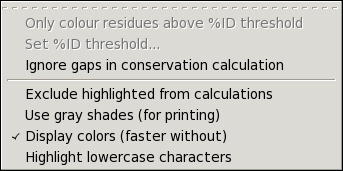
\includegraphics[width=9.3cm]{img_menu_settings.png}
\caption{Settings menu}
\label{fig:settings_menu}
\end{figure}

\begin{supertabular}{>{\bfseries}p{0.4\textwidth} p{0.6\textwidth}}
Only colour residues above \%ID threshold &
Only applicable in colour-by-residue mode; only colour residues that have a percent identity above the threshold specified by the {\textquotesingle}Set \%ID threshold{\textquotesingle} menu option\\
Ignore gaps in conservation calculation &
Only applicable in colour-by-conservation mode; ignore gaps when calculating the conservation\\
Exclude highlighted from calculations &
Exclude the currently-selected row from colour calculations\\
Use gray shades &
Only applicable to colour-by-conservation mode; use grey shades (suitable for printing)\\
Display colours &
Whether to show colours or not (faster without)\\
Highlight lowercase characters &
Highlights lowercase characters\\
\end{supertabular}


\subsection[Help menu]{Help menu}



\begin{figure}[htb]
\centering
\color{lightblue}

\includegraphics[width=0.3\textwidth]{img_menu_help.png}
\caption{Help menu}
\label{fig:help_menu}
\end{figure}

\begin{supertabular}{>{\bfseries}l l}
Help &
Show the help pages\\
About &
Show the {\textquotesingle}About{\textquotesingle} dialog\\
\end{supertabular}


\clearpage\section[Keyboard shortcuts]{Keyboard shortcuts}

Recommended shortcuts (consistent with other SeqTools programs):
 
\begin{supertabular}{>{\bfseries}p{0.2\textwidth} p{0.8\textwidth}}
,

. &
Scroll one column left

Scroll one column right\\
Ctrl-,

Ctrl-. &
Scroll one page left

Scroll one page right\\
Shift-Ctrl-,

Shift-Ctrl-. &
Scroll to leftmost column

Scroll to rightmost column\\
PageUp

PageDown &
Scroll one page up

Scroll one page down\\
Ctrl-up

Ctrl-down &
Scroll one row up

Scroll one row down\\
Home

End &
Scroll to top of alignment list

Scroll to bottom of alignment list\\
Ctrl-W &
Close the current window. \ If this is the main window, it quits the application\\
Ctrl-Q &
Quit the application\\
Ctrl-S &
Save the alignment in the current format\\
Shift-Ctrl-S &
Save the alignment in a different format\\
Ctrl-P &
Print the current window\\
Ctrl-H &
Open the Help pages\\
Ctrl-F &
Find sequences\\
Ctrl-R &
Make non-redundant\\
Ctrl-T &
Remove partial sequences\\
t &
Toggle between colour-by-residue and colour-by-conservation mode\\
= (equal) &
Zoom in\\
{}- (minus) &
Zoom out\\
\end{supertabular}

Old-style Belvu shortcuts:

\begin{supertabular}{>{\bfseries}p{0.2\textwidth} p{0.8\textwidth}}
Left-arrow

Right-arrow &
Scroll one page left

Scroll one page right\\
Ctrl-left

Ctrl-right &
Scroll one column left

Scroll one column right\\
Up-arrow

Down-arrow &
Scroll one page up

Scroll one page down\\
Insert

Delete &
Scroll to leftmost column

Scroll to rightmost column\\
\end{supertabular}


\end{document}
